\documentclass[12pt, a4paper, oneside]{ctexart}
\usepackage{amsmath, amsthm, amssymb, bm, color, graphicx, geometry, mathrsfs,extarrows, braket, booktabs, array, xcolor, fontspec, appendix, float, subfigure, wrapfig, enumitem}
\usepackage[colorlinks,linkcolor=red,anchorcolor=blue,citecolor=blue,urlcolor=blue,menucolor=black]{hyperref}

%%%% 设置中文字体 %%%%
\setCJKmainfont{方正新书宋_GBK.ttf}[BoldFont = 方正小标宋_GBK, ItalicFont = 方正楷体_GBK, BoldItalicFont = 方正粗楷简体]
%%%% 设置英文字体 %%%%
\setmainfont{Times New Roman}
\setsansfont{Calibri}
\setmonofont{Consolas}

%%%% 设置代码块 %%%%
% 在vscode中使用minted需要先配置python解释器, Ctrl+Shift+P, 输入Python: Select Interpreter选择安装了Pygments的Python版本. 再在setting.json中xelatex和pdflatex的参数中加入 "--shell-escape", 即可
% TeXworks中配置方法参考: https://blog.csdn.net/RobertChenGuangzhi/article/details/108140093
\usepackage{minted}
\renewcommand{\theFancyVerbLine}{
    \sffamily\textcolor[rgb]{0.5,0.5,0.5}{\scriptsize\arabic{FancyVerbLine}}} % 修改代码前序号大小
% 加入不同语言的代码块
\newmintinline{cpp}{fontsize=\small, linenos, breaklines, frame=lines}
\newminted{cpp}{fontsize=\small, linenos, breaklines, frame=lines}
\newmintedfile{cpp}{fontsize=\small, linenos, breaklines, frame=lines}
\newmintinline{matlab}{fontsize=\small, linenos, breaklines, frame=lines}
\newminted{matlab}{fontsize=\small, mathescape, linenos, breaklines, frame=lines}
\newmintedfile{matlab}{fontsize=\small, linenos, breaklines, frame=lines}
\newmintinline{python}{fontsize=\small, linenos, breaklines, frame=lines, python3}  % 使用\pythoninline{代码}
\newminted{python}{fontsize=\small, linenos, breaklines, frame=lines, python3}  % 使用\begin{pythoncode}代码\end{pythoncode}
\newmintedfile{python}{fontsize=\small, linenos, breaklines, frame=lines, python3}  % 使用\pythonfile{代码地址}

%%%% 设置行间距与页边距 %%%%
\linespread{1.2}
\geometry{left=2.5cm, right=2.5cm, top=2.5cm, bottom=2.5cm}

%%%% 定理类环境的定义 %%%%
\newtheorem{example}{例}            % 整体编号
\newtheorem{theorem}{定理}[section] % 定理按section编号
\newtheorem{definition}{定义}
\newtheorem{axiom}{公理}
\newtheorem{property}{性质}
\newtheorem{proposition}{命题}
\newtheorem{lemma}{引理}
\newtheorem{corollary}{推论}
\newtheorem{condition}{条件}
\newtheorem{conclusion}{结论}
\newtheorem{assumption}{假设}
\numberwithin{equation}{section}  % 公式按section编号 (公式右端的小括号)
\newtheorem{algorithm}{算法}

\newsavebox{\nameinfo}
\newenvironment{myTitle}[1]{
    \begin{center}
    {\zihao{-2}\bf #1\\}
    \zihao{-4}\it
}{\end{center}}  % \begin{myTitle}{标题内容}作者信息\end{myTitle}
\newcounter{problem}  % 问题序号计数器
\newenvironment{problem}[1][]{\stepcounter{problem}\par\noindent\textbf{题目\arabic{problem}. #1}}{\smallskip\par}
\newenvironment{solution}[1][]{\par\noindent\textbf{#1解答. }}{\smallskip\par}  % 可带一个参数表示题号\begin{solution}{题号}
\newenvironment{note}{\par\noindent\textbf{注记. }}{\smallskip\par}
\newenvironment{remark}{\begin{enumerate}[label=\textbf{注\arabic*.}]}{\end{enumerate}}

%%%% 图片相对路径 %%%%
\graphicspath{{figure/}} % 当前目录下的figure文件夹, {../figure/}则是父目录的figure文件夹
\setlength{\abovecaptionskip}{-0.2cm}  % 缩紧图片标题与图片之间的距离
\setlength{\belowcaptionskip}{0pt} 

%%%% 缩小item,enumerate,description两行间间距 %%%%
\setenumerate[1]{itemsep=0pt,partopsep=0pt,parsep=\parskip,topsep=5pt}
\setitemize[1]{itemsep=0pt,partopsep=0pt,parsep=\parskip,topsep=5pt}
\setdescription{itemsep=0pt,partopsep=0pt,parsep=\parskip,topsep=5pt}

\everymath{\displaystyle} % 默认全部行间公式, 想要变回行内公式使用\textstyle
\DeclareMathOperator*\uplim{\overline{lim}}     % 定义上极限 \uplim_{}
\DeclareMathOperator*\lowlim{\underline{lim}}   % 定义下极限 \lowlim_{}
\DeclareMathOperator*{\argmax}{arg\,max}  % 定义取最大值的参数 \argmax_{}
\DeclareMathOperator*{\argmin}{arg\,min}  % 定义取最小值的参数 \argmin_{}
\let\leq=\leqslant % 简写小于等于\leq (将全部leq变为leqslant)
\let\geq=\geqslant % 简写大于等于\geq (将全部geq变为geqslant)
\DeclareRobustCommand{\rchi}{{\mathpalette\irchi\relax}}
\newcommand{\irchi}[2]{\raisebox{\depth}{$#1\chi$}} % 使用\rchi将\chi居中

%%%% 一些宏定义 %%%%
\def\bd{\boldsymbol}        % 加粗(向量) boldsymbol
\def\disp{\displaystyle}    % 使用行间公式 displaystyle(默认)
\def\tsty{\textstyle}       % 使用行内公式 textstyle
\def\sign{\text{sign}}      % sign function
\def\wtd{\widetilde}        % 宽波浪线 widetilde
\def\R{\mathbb{R}}          % Real number
\def\N{\mathbb{N}}          % Natural number
\def\Z{\mathbb{Z}}          % Integer number
\def\Q{\mathbb{Q}}          % Rational number
\def\C{\mathbb{C}}          % Complex number
\def\K{\mathbb{K}}          % Number Field
\def\P{\mathbb{P}}          % Polynomial
\def\N{\mathbb{N}}          % Natural number
\def\Z{\mathbb{Z}}          % Integer number
\def\E{\mathbb{E}}          % Exception
\def\var{\text{Var}}        % Variance
\def\cov{\text{Cov}}        % Coefficient of Variation
\def\bias{\text{bias}}      % bias
\def\d{\mathrm{d}}          % differential operator
\def\e{\mathrm{e}}          % Euler's number
\def\i{\mathrm{i}}          % imaginary number
\def\re{\mathrm{Re}}        % Real part
\def\im{\mathrm{Im}}        % Imaginary part
\def\res{\mathrm{Res}}      % Residue
\def\L{\mathcal{L}}         % Loss function
\def\O{\mathcal{O}}         % 时间复杂度
\def\wdh{\widehat}          % 宽帽子 widehat
\def\ol{\overline}          % 上横线 overline
\def\ul{\underline}         % 下横线 underline
\def\add{\vspace{1ex}}      % 增加行间距
\def\del{\vspace{-1.5ex}}   % 减少行间距

%%%% 正文开始 %%%%
\begin{document}
\begin{myTitle}{CVPR第四次作业-Caltech256数据集图像分类}
    强基数学\\
    吴天阳\quad 2204210460,陈开来\quad 2205110920,王瑞恒\quad 2202113454,\\
    马煜璇\quad 2204220461,申宇环\quad 2201422097
\end{myTitle}
\section{实验目的}
基于Caltech256数据集的深度网络分类性能比较.

\begin{enumerate}
    \item 以Caltech256为试验数据集,按照原始数据集的要求进行训练、测试集的划分.
    \item 比较不少于三种深度神经网络结构,全部\textbf{平均精度}不低于85\%.
    \item 对算法从处理速度、正确率方面给出性能评估.
\end{enumerate}

我们选择了VGG-19,Inception-ResNet,MoblieNet,EfficientNet对Caltech256数据集进行测试,并对其进行评估. 首先介绍卷积神经网络基本原理和6大经典模型的特点.
\section{实验原理}
\subsection{卷积神经网络基础}
这里的卷积指的是\textbf{离散型}的卷积形式.

\subsubsection{一维卷积}

设 \(\{w_i\},\{x_i\}\) 为两个数列,\(k\in\mathbb{R}\),定义 \(\{w_i\}\)
与 \(\{x_i\}\) 的有限卷积为以下数列
\begin{equation}\label{eq-conv0}
   y_t = \sum_{k=1}^Kw_kx_{t-k+1},\quad(t\geqslant K) 
\end{equation}
其中 \(\{w_i\}\) 称为\textbf{滤波器}(Filter)或卷积核(Convolution
Kernel),\(\{x_i\}\) 为\textbf{信号序列},\(K\) 为\textbf{滤波器长度}.

如果我们将数列记为对应的函数值:\(w(i) = w_i\ (1\leqslant i\leqslant K),\ x(i) = x_i\ (1\leqslant i),\ y(t) = y_t\ (K\leqslant t)\).
则上述定义可视为:数列 \(\{w_i\}, \{x_i\}\) 在 \(\mathbb{R}\)
上的零延拓,即
\(w(i) = \begin{cases}w_i,&\quad1\leqslant i\leqslant K,\\0,&\quad\texttt{otherwise}.\end{cases}\)
用更形象的方式将其列出如下

\begin{equation*}
    \addtocounter{MaxMatrixCols}{11}
    \begin{matrix}
        i=&\cdots,&-1,&0,&1,&2,&\cdots,&K,&K+1,&K+2,&\cdots\\
        w(i)=&\cdots,&0,&w_1,&w_2,&w_3,&\cdots,&w_K,&0,&0,&\cdots\\
        x(i)=&\cdots,&0,&x_1,&x_2,&x_3,&\cdots,&x_K,&x_{K+1},&x_{K+2},&\cdots
    \end{matrix}
\end{equation*}

定义两个离散数列 \(\{w_i\},\{x_i\}\) 的卷积如下:
\begin{align}
    \label{eq-conv1}w*x :=&\ \sum_{i=-\infty}^\infty w_ix_{t-i+1}\xlongequal{i = t-j+1}\sum_{j=-\infty}^\infty x_jw_{t-j+1}=x * w\\
    \label{eq-conv2}=&\ \sum_{i=1}^Kw_ix_{t-i+1}
\end{align}

通过(\ref{eq-conv1})式可知卷积具有可交换性,(\ref{eq-conv2})式表明(\ref{eq-conv0})式中定义的有限卷积其实就是在数列零延拓下的卷积,再截取 \(t\geqslant K\)
这一段的结果.

卷积操作在信号处理方面有不错的效果,可以通过不同的卷积核,对不同的信号进行提取.
下面是几个简单例子.

\begin{enumerate}
\def\labelenumi{\arabic{enumi}.}
\item
  简单移动平移:\(w = [1/k,\ 1/k,\ \cdots,\ 1/k]\)(用于时间序列中消除数据的随机波动).
\item
  二阶微分近似:\(w=[1,\ -2,\ 1]\),由数值分析的知识可知,连续二阶可微函数
  \(x(t)\),有如下近似式
  \[x''(t) \approx \frac{x(t-h)-2x(t)+x(t+h)}{h^2}\xlongequal{\text{令}h=1}x(t-1)-2x(t)+x(t+1)\]
\end{enumerate}

\subsubsection{二维卷积}

常用于图像处理,设图像 \(x\in\mathbb{R}^{M\times N}\) ,卷积核
\(w\in\mathbb{R}^{U\times V}\),一般有
\(U\ll M,V\ll N\),类比一维卷积定义,二维卷积定义如下:
\begin{equation}\label{eq-2Dconv}
   y_{st} = \sum_{i=1}^U\sum_{j=1}^Vw_{ij}x_{s-i+1,t-j+1}=\sum_{i=-\infty}^\infty\sum_{j=-\infty}^\infty w'_{ij}x'_{s-i+1,t-j+1}=:w*x 
\end{equation}
其中 \(w'_{ij}, x'_{ij}\) 分别为 \(w_{ij}, x_{ij}\) 的零延拓,记
\(y=w * x\in\mathbb{R}\). 图\ref{fig-diff-kernel}是几种不同卷积核作用在一张图片上的效果.
\begin{figure}[htbp]
    \centering
    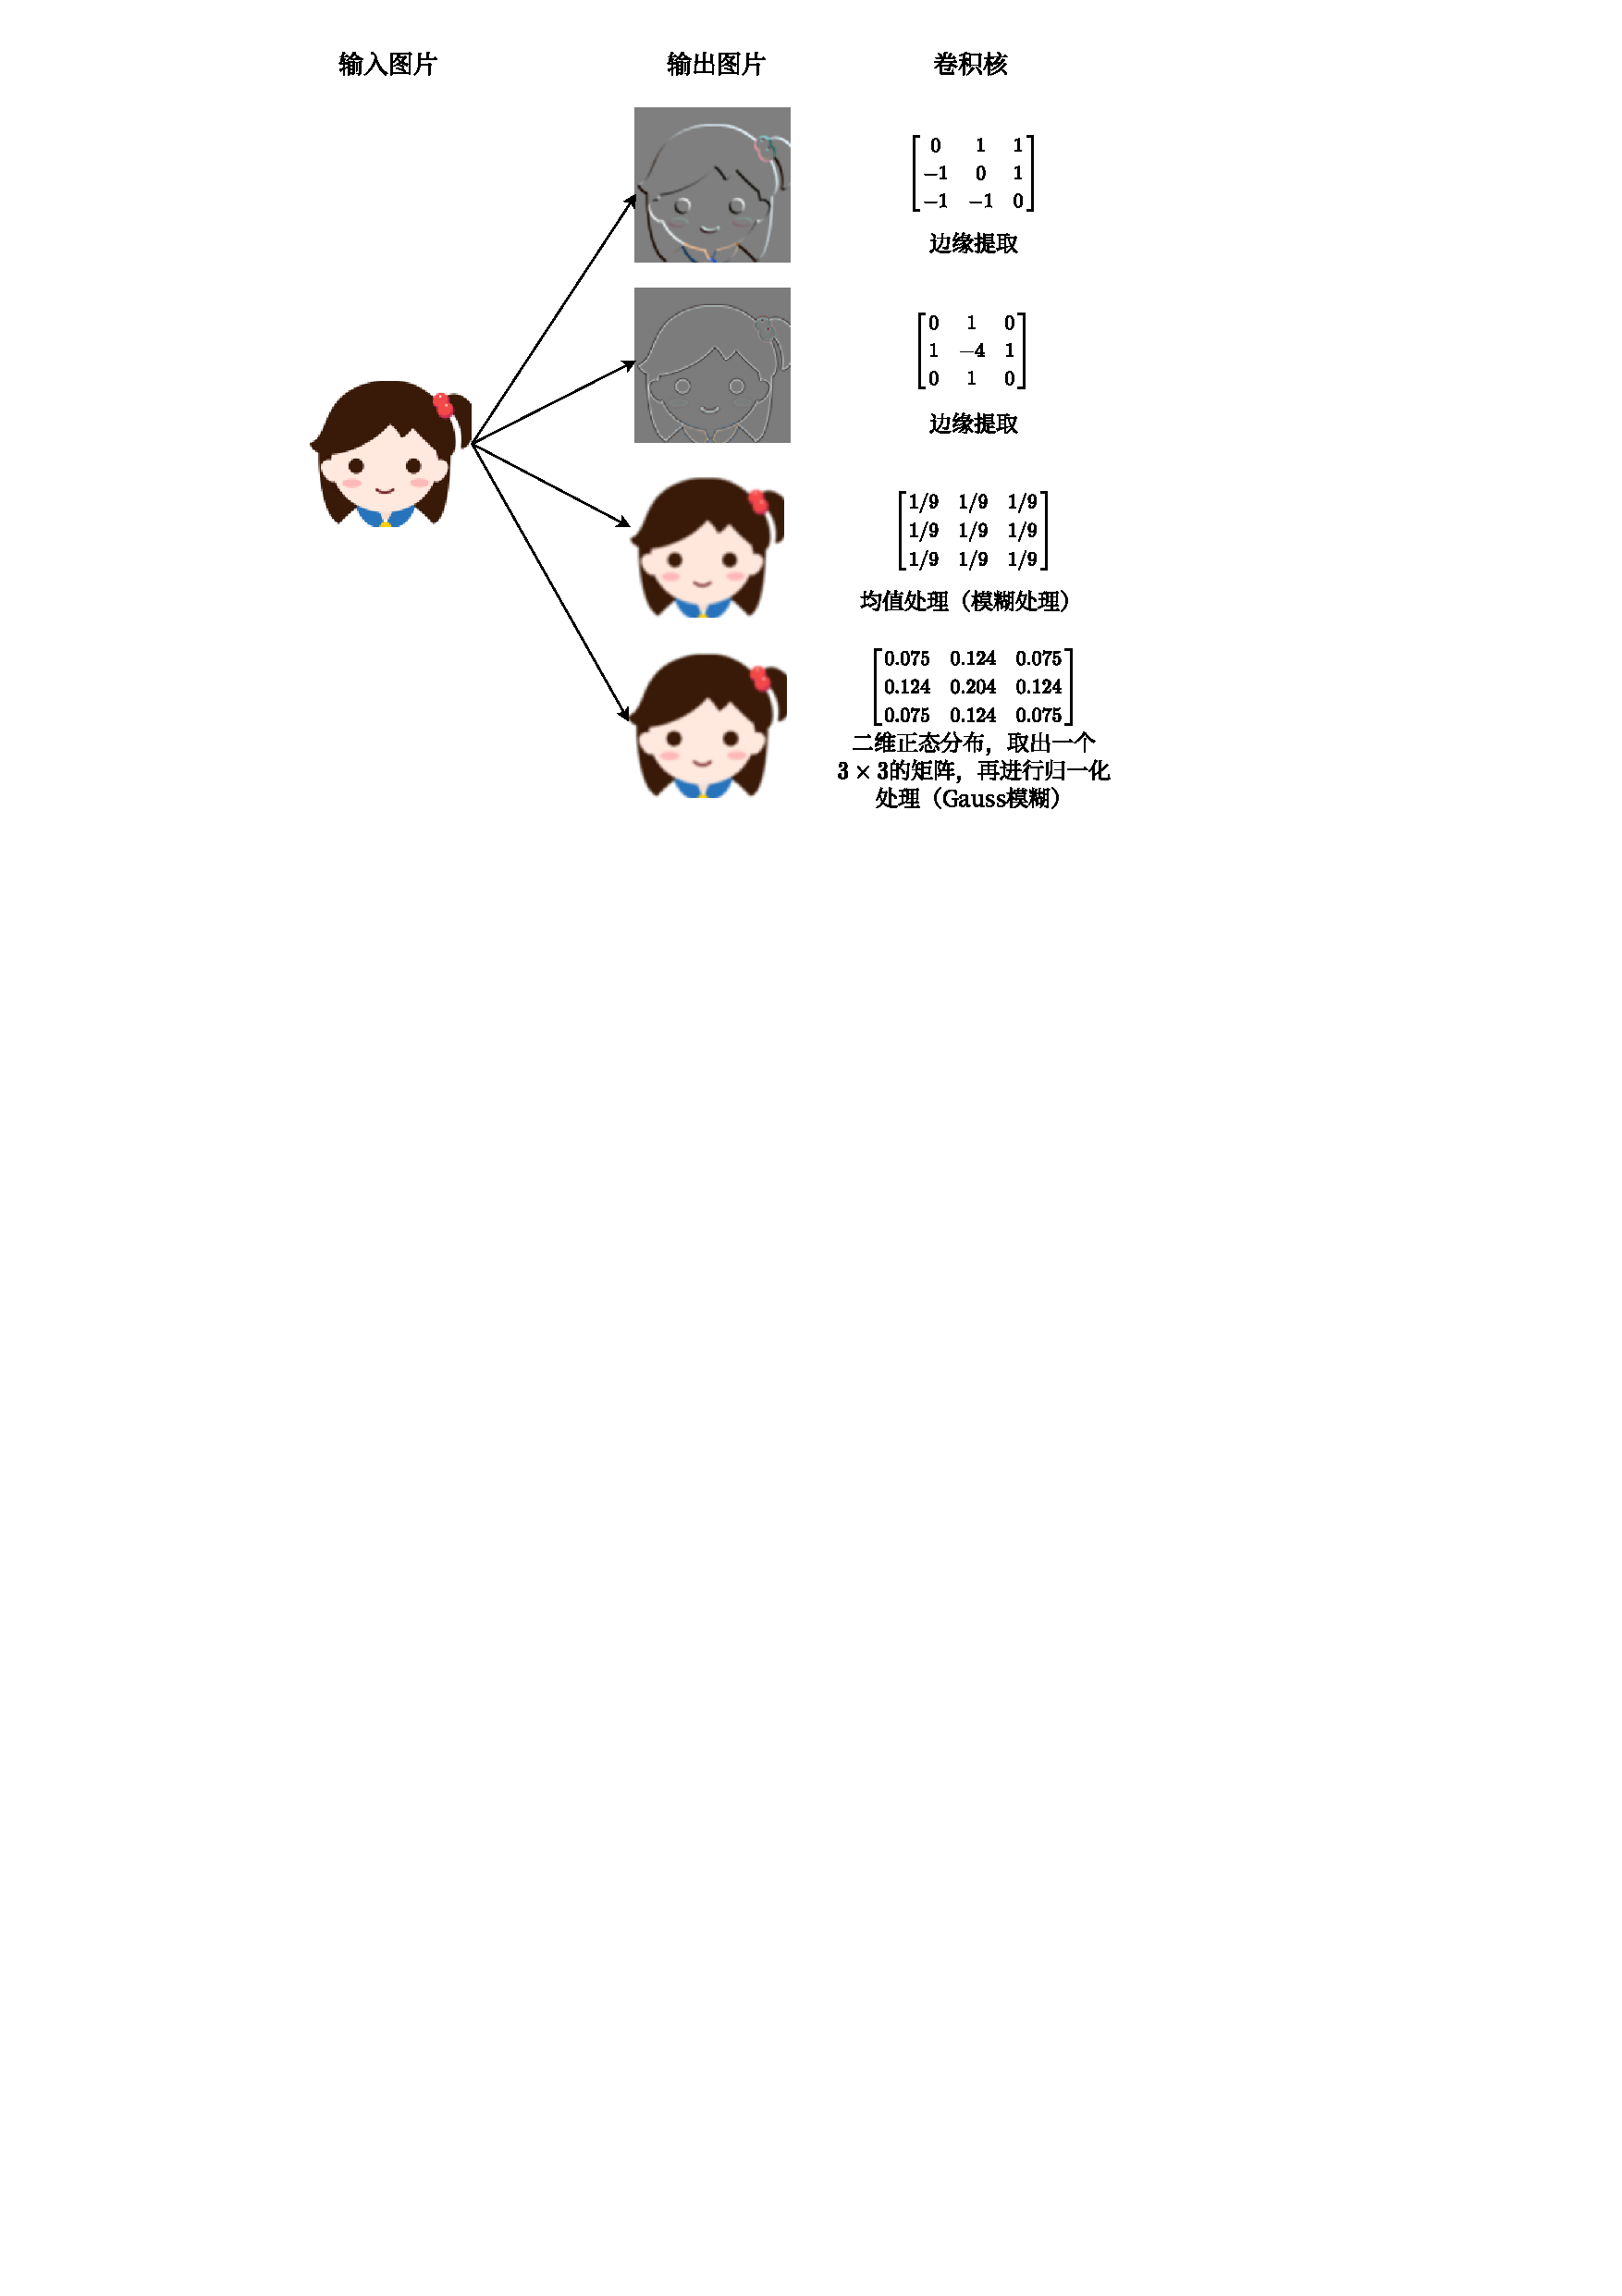
\includegraphics[scale=0.8]{differnt kernel.drawio.pdf}
    \caption{不同卷积核处理效果}
    \label{fig-diff-kernel}
\end{figure}

\subsubsection{互相关}

在机器学习和图像处理中,卷积的作用主要是通过在一个图像上滑动一个卷积核,通过卷积操作得到一个新的图像.
在计算卷积过程中,需要对卷积核进行反转操作,即对卷积核旋转 \(\pi\) 大小.
这个操作就显得多余了,所以在计算机中经常将卷积视为\textbf{互相关}(Cross-Correlation)操作,即直接对卷积核和原图进行点积操作(对应位相乘).

设图像 \(x\in\mathbb{R}^{M\times N}\) ,卷积核
\(w\in\mathbb{R}^{U\times V}\),则它们的互相关为:
\begin{equation}
   y_{st} = \sum_{i=1}^U\sum_{j=1}^Vw_{ij}x_{s+i-1,t+j-1} = \sum_{i=-\infty}^\infty\sum_{j=-\infty}^\infty w'_{ij}x'_{s+i-1,t+j-1}=:w\otimes x 
\end{equation}
和(\ref{eq-2Dconv})式对照可知,互相关和卷积的区别仅仅在于卷积核是否需要翻转,即
\(w\otimes x = \text{rot}(w)*x\),\(\text{rot}(w)\) 表示将矩阵 \(w\)
旋转 \(\pi\) 以后的结果. 因此互相关也称为不翻转卷积.

\subsubsection{卷积的变种}

在卷积的基础上,还可以引入步长和零填充增加卷积的多样性,以便更灵活地提取图像特征.

\begin{itemize}
\item
  \textbf{步长}(Stride)指卷积核在滑动时的时间间隔. 如图\ref{fig-stride-zeropadding}(a).
\item
  \textbf{零填充}(Zero Padding)指对输入矩阵的边缘进行零填充. 如图\ref{fig-stride-zeropadding}(b).
\end{itemize}

\begin{figure}[htbp]
    \centering
    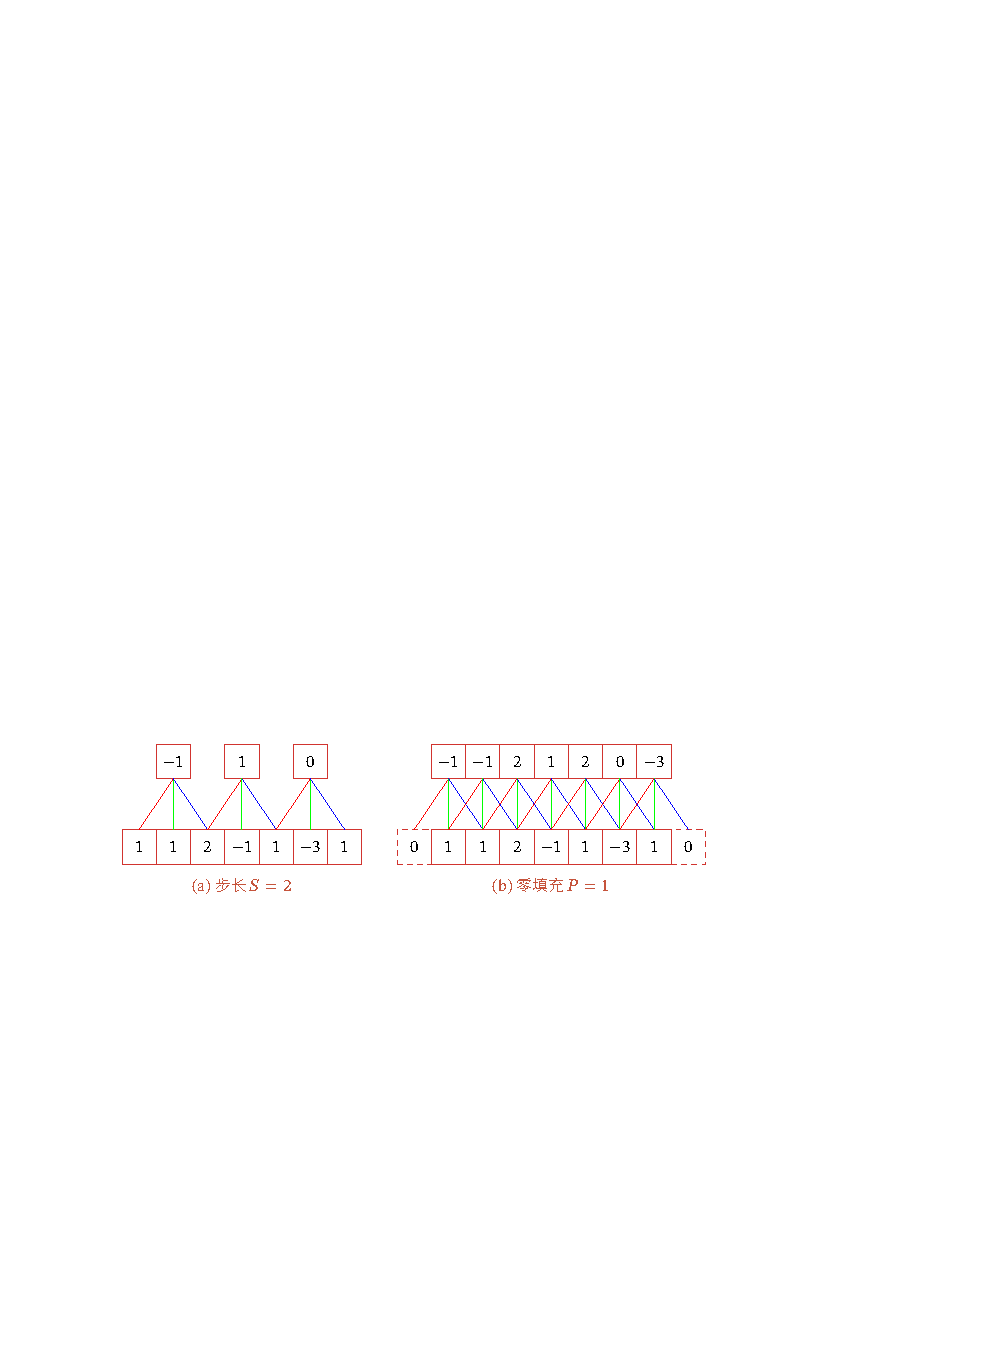
\includegraphics[scale=1.2]{步长和零填充.pdf}
    \caption{步长和零填充}
    \label{fig-stride-zeropadding}
\end{figure}

设卷积层的输入向量维数为 \(M\),卷积大小为 \(K\),步长为
\(S\),在输入两端各填补 \(P\) 个 \(0\),则输出向量维度为
\((M-K+2P)/S+1\),

常用卷积有以下三种:

\begin{enumerate}
\def\labelenumi{\arabic{enumi}.}
\item
  \textbf{窄卷积}(Narrow Convolution):\(S=1, P=0\),输出维度为
  \(M-K+1\).(普通卷积)
\item
  \textbf{宽卷积}(Wide Convolution): \(S=1, P=K-1\),输出维度为
  \(M+K-1\).
\item
  \textbf{等宽卷积}(Equal-Width
  Convolution):\(S=1, P=(K-1)/2\),输出维度为 \(K\).
  如图\ref{fig-stride-zeropadding}(b)就是一种等宽卷积.
\end{enumerate}

\subsection{卷积神经网络结构}
\subsubsection{卷积层}

卷积层的作用是提取局部区域的特征,将输入卷积层的矩阵称为\textbf{输入特征},将通过卷积层后的输出称为\textbf{输出特征},也称\textbf{特征映射}(Feature
Map).

一般的图片每个像素由RGB三原色(颜色通道数为
\(3\))构成,假设图片的宽度和高度分别为 \(N, M\),颜色通道数为
\(D\),则一张图片
\(x\in\mathbb{R}^{N\times M\times D}\),由于图片的像素值一般为无符号
\(8\) 位整型,即 \(x_{ijk}\in[0,255]\),所以也有
\(x\in[0,255]^{N\times M\times D}\),当我们对图片进行\textbf{归一化处理}后,即
\(x\leftarrow x / 256\),就有 \(x\in[0, 1)^{N\times M\times D}\).

卷积层中,假设每个卷积核大小为 \(U\times V\),且每个颜色通道上都对应有
\(P\) 个卷积核,则卷积核
\(w\in\mathbb{R}^{U\times V\times P\times D}\),令第 \(d\)
个颜色通道上的第 \(p\)个卷积核为 \(w_{d,p}\). 由于每个卷积核 \(w_{d,p}\)
作用在图片 \(x\) 上都会得到一个输出 \(y_p\),所以一共有 \(P\)
个输出特征,所以特征映射
\(y\in\mathbb{R}^{N'\times M'\times P}\),\(N'\times M'\) 为卷积核
\(U\times V\) 作用在 \(N\times M\) 矩阵后的维度. 可以参考下图更好地理解.
\begin{figure}[htbp]
    \centering
    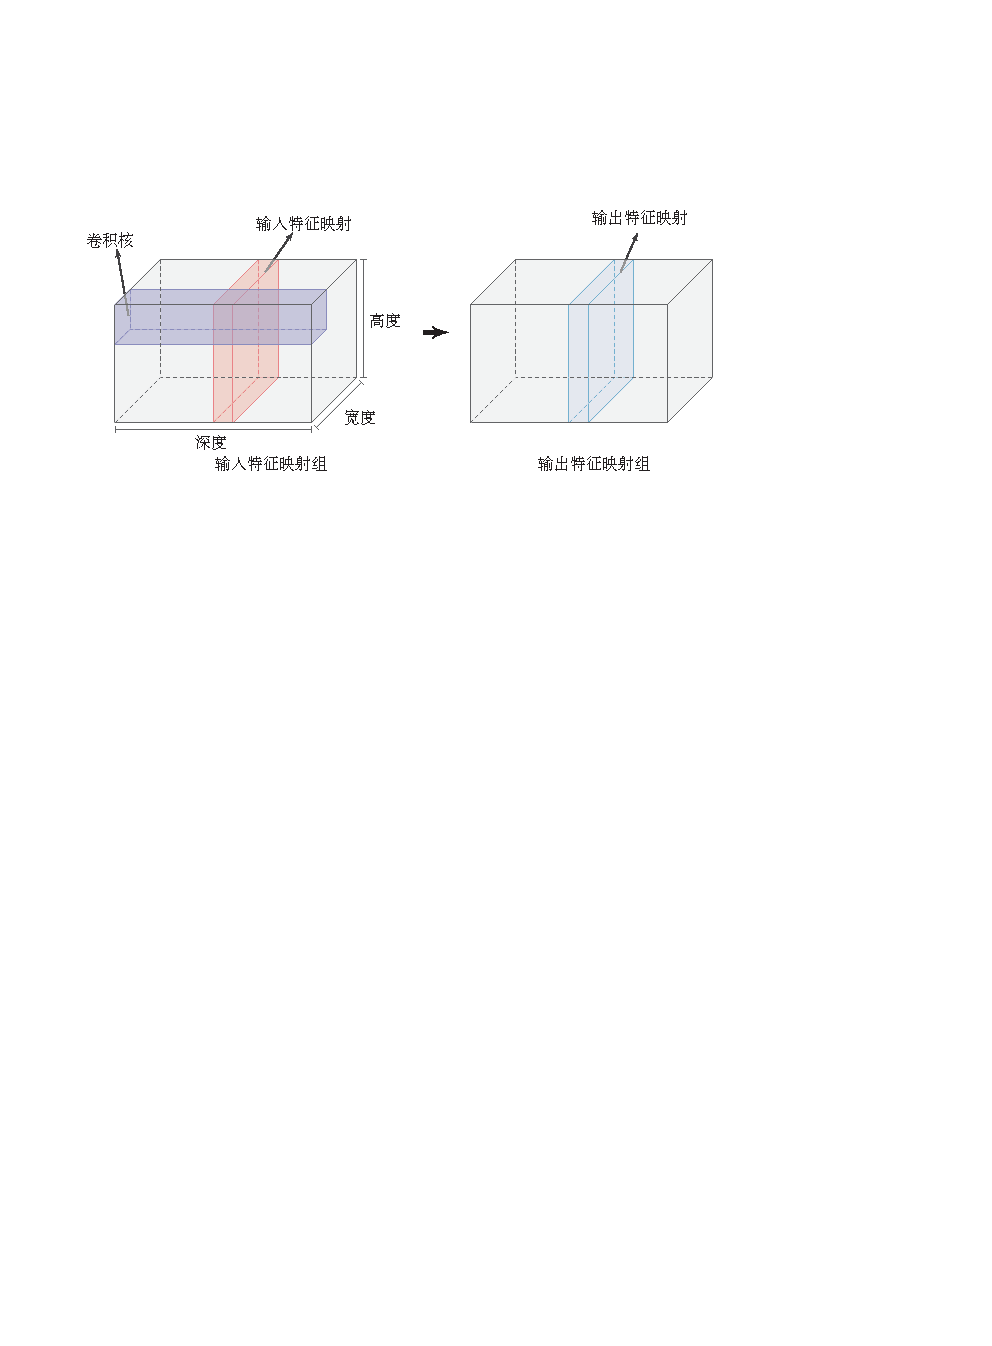
\includegraphics[scale=1.4]{卷积层的三维结构.pdf}
    \caption{卷积层的三维结构}
    \label{fig-conv-struct}
\end{figure}
\subsubsection{汇聚层}

\textbf{汇聚层}(Pooling
Layer)也称\textbf{池化层},\textbf{子采样层}(Subsampling Layer).
起作用是对卷积层输出的特征映射进一步进行特征选取,降低特征数量,减少参数数量.

设汇聚层的输入特征
\(x\in\mathbb{R}^{N\times M\times D}\),对于其中每一个颜色通道中的图像
\(x^d\),划分为很多的区域 \(\{R_{ij}^d\}\),满足
\(\bigcup_{ij} R_{ij}^d\subset\{x_{ij}\}\),这些区域可以是不交的,也可以有交集.
\textbf{汇聚}(Pooling)是指对每个区域进行\textbf{下采样}(Down
Sampling)操作得到的值,作为该区域的概括.

常用的汇聚操作有以下两种:
\begin{enumerate}
\def\labelenumi{\arabic{enumi}.}
\item
  \textbf{最大汇聚}(Maximum Pooling):对于一个区域
  \(R^d_{ij}\),选择这个区域内所有神经元的最大活性值作为这个区域的表示,即
  \begin{equation}
    y^d_{ij} = \max_{x\in R^d_{ij}}x
  \end{equation}
\item
  \textbf{平均汇聚}(Mean
  Pooling):取该区域内的所有活性值的平均值作为该区域的表示,即
  \begin{equation}
    y_{ij}^d=\frac{1}{|R_{ij}^d|}\sum_{x\in R_{ij}^d}x
  \end{equation}
  其中 \(|R_{ij}^d|\) 表示集合 \(R_{ij}^d\)
  的基数,即该集合中所包含元素的个数.
\end{enumerate}

\subsubsection{卷积网络的一般结构}

一个经典卷积网络由卷积层、汇聚层、全连接层堆叠而成,常用卷积神经网络结构如图\ref{fig-classicCNN}所示.
一个\textbf{卷积块}为一组连续 \(M\) 个卷积层和 \(b\) 个汇聚层构成(\(M\)
取值通常为 \(2\sim 5\),且卷积核大小逐层增大,个数逐层增多,\(b\)
通常取为 \(0\) 或 \(1\)),卷积神经网络堆叠 \(N\)
个连续的卷积块,然后连接 \(K\) 个全连接层(\(N\) 通常取为 \(1\sim 100\)
或更大,\(K\) 一般取为 \(0\sim 2\)).
\begin{figure}[htbp]
    \centering
    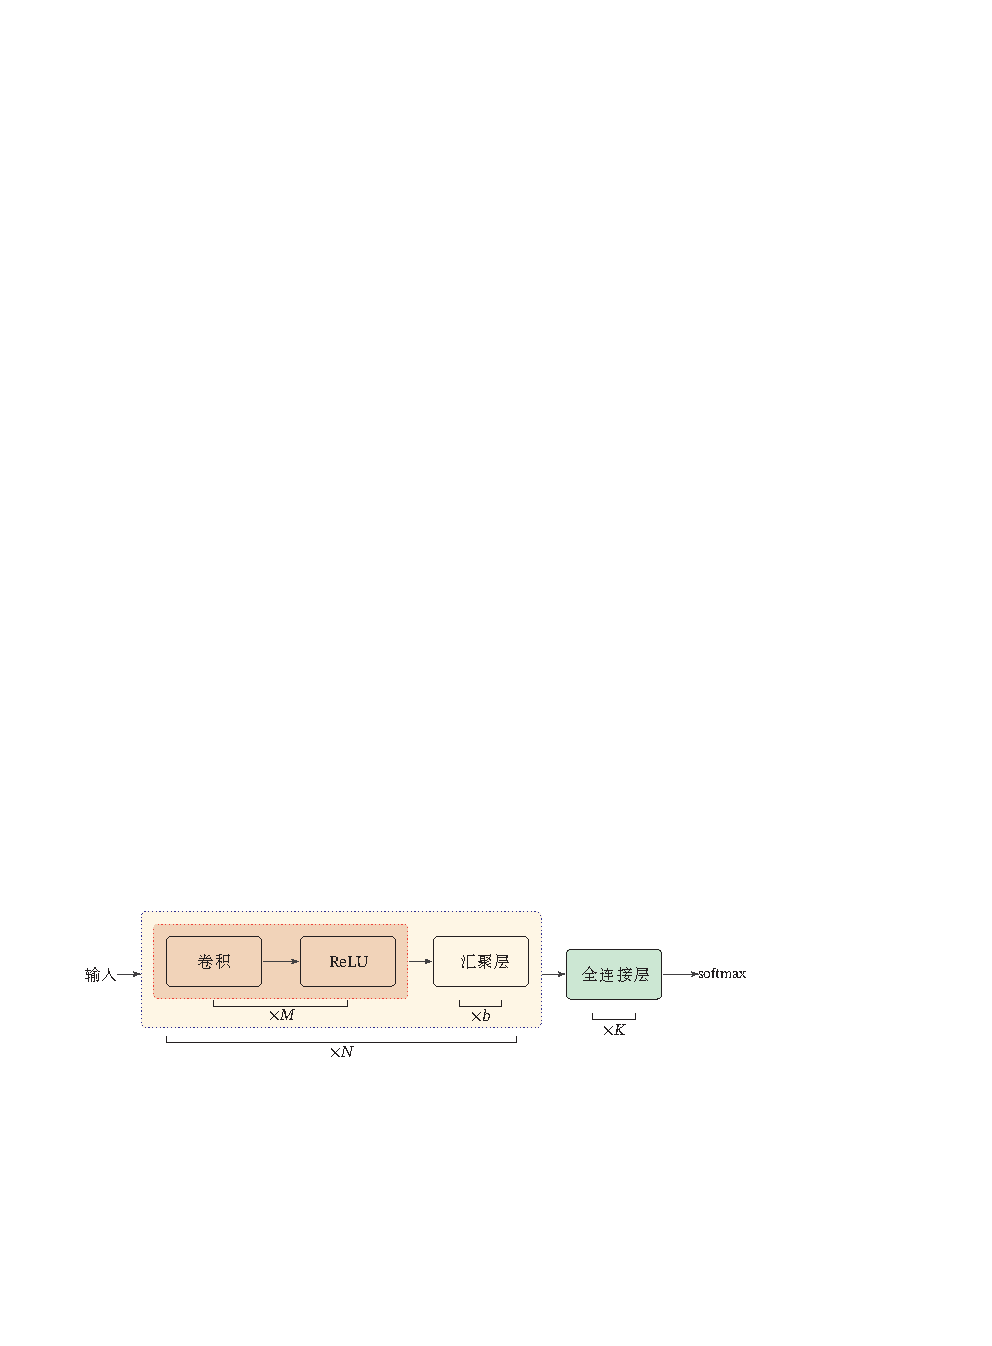
\includegraphics[scale=1.4]{经典卷积网络结构.pdf}
    \caption{经典卷积网络结构}
    \label{fig-classicCNN}
\end{figure}

卷积网络的卷积核大小一般取为 \(2\times 2\) 或
\(3\times 3\),以及更多的数量如 \(32\) 个或更多.
由于卷积可以设置步长减少输出特征的大小,所以汇聚层的作用并不显著了,可以通过增加步长来替代.

\subsection{经典图像分类网络原理}
\subsubsection{AlexNet}
AlexNet夺得了2012年\href{https://image-net.org/challenges/LSVRC/}{ImageNet比赛}第一名,是最经典的卷积神经网络模型,使用$227\times 227$的图像输入,论文中中画的是$224\times 224$,后来指出应该是通过padding增加到了$227\times 227$的输入. $5$个卷积层,$3$个最大池化层,$3$个全连接层,前两个激活函数使用ReLU,最后一层使用softmax转化为概率值进行分类. 具体网络结构见图\ref{fig-AlexNet}.

参考论文:\href{https://proceedings.neurips.cc/paper/2012/file/c399862d3b9d6b76c8436e924a68c45b-Paper.pdf}{ImageNet Classification with Deep Convolutional Neural Networks - 2012}.
\begin{figure}[htbp]
  \centering
  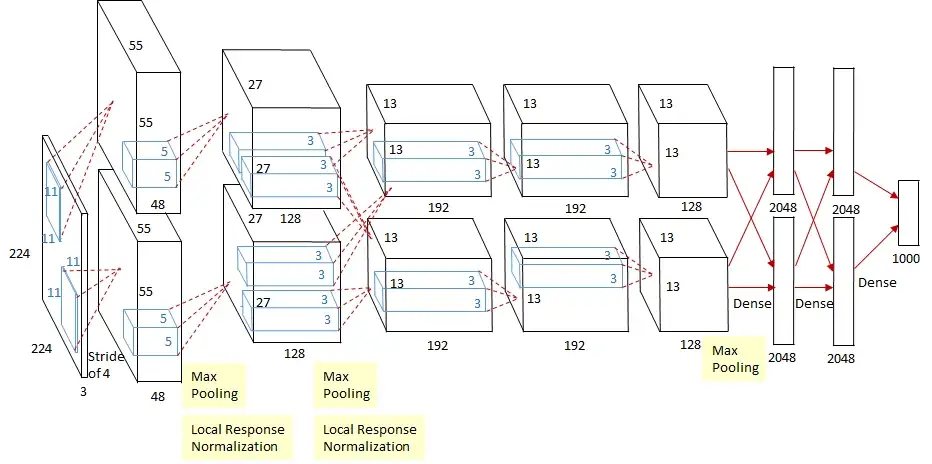
\includegraphics[scale=0.48]{AlexNet.png}
  \caption{AlexNet基本结构}
  \label{fig-AlexNet}
\end{figure}

AlexNet特点具有的特点:

\textbf{1. ReLU激活函数}:在AlexNet之前,神经网络使用的一般为tanh作为激活函数,而AlexNet中使用的全部为ReLU激活函数,论文中显示,达到相同的75\%正确率下,ReLU比tanh快接近6倍的时间.

\textbf{2. GPU多线程处理}:当时训练所使用的的显卡为NVIDIA GTX 580 GPU,仅有3GB显存,为了避免显存超出,在神经网络框架上可以看出,图像被划分为两条路径分别进行卷积操作,但并没有实现速度上的提升. 现在的显卡控制好batch大小,已经不会再出现显存溢出问题了.

\textbf{3. 局部响应归一化}:对局部值的特征进行了归一化操作,归一化操作可以提升神经网络收敛速度,而现在神经网络使用的更多的是以batch作为一个单位进行归一化操作.

\textbf{4. 数据增强}:主要是使用了如下两种数据增强方法:图像平移与水平翻转,改变光照强度.

\textbf{5. Dropout}:Dropout操作是指每次训练过程中会随机丢弃一定比例的神经元,并且不进行梯度更新;在测试集上运行时,则不会调用Dropout操作. 该操作是一种正则化操作,使得每个神经元都有更大的概率去更新权重,可以一定程度上避免过拟合发生.

\subsubsection{VGG}
VGG神经网络是2014年ImageNet比赛中的第二名. 参考论文:\href{https://arxiv.org/pdf/1409.1556.pdf}{Very Deep Convolutional Networks for Large-Scale Image Recognition - 2014}.

VGG是在AlexNet上的进一步改进. 在VGG神经网络中,卷积层持续使用大小为$3\times 3$,步长为$1$,padding为$1$的卷积核;所有池化层均为最大池化层,大小为$2\times 2$,步长为$2$,在通过池化层之后通道数加倍.


VGG网络共包含5个卷积阶段:

阶段1:conv-conv-pool

阶段2:conv-conv-pool

阶段3:conv-conv-pool

阶段4:conv-conv-conv-[conv]-pool

阶段5:conv-conv-conv-[conv]-pool

\textbf{注}:在VGG-19中阶段4,5中包含4个卷积层.

VGG的设计思路主要是:相同的卷积核大小,在使用更小更多的卷积核与一个大卷积核的感受野形同,但具有更少的参数和计算量,所以VGG中全部使用了$3\times 3$的卷积核代替$5\times 5$的卷积核.

缺点:VGG-16的内存开销整体上比AlexNet大了$25$倍,参数增多了$2.3$倍,整体训练难度提高.

\subsubsection{GoogleNet}
GoogleNet在2014年ImageNet比赛的第一名,在随后的两年后一直改进,产生了Inception V2、Inception V3、Inception V4(Inception-Resnet)众多版本,最后的一个版本我们还会对其进行介绍,并用其做本次图像识别任务. 参考论文:\href{https://arxiv.org/abs/1409.4842}{Going Deeper with Convolutions - 2014}

提升网络识别图像的性能一般是增加网络的深度和宽度,但是直接增加会产生非常多问题:

\begin{enumerate}
  \item 参数太多,若训练集有限,容易过拟合;
  \item 网络越大,训练难度增加,计算复杂度增大,难以应用;
  \item 网络越深,容易发生梯度消失问题,难以优化模型.
\end{enumerate}

希望在增加网络深度和宽度的同时减少参数,通过将全连接转化为稀疏连接从而减少参数个数,这里稀疏连接指的就是池化层,在GoogleNet中\textbf{使用了平均池化层代替输出层前的多个全连接层},大大减少了参数数目;并提出Inception方法就是把多个卷积或池化操作组装为一个网络模块,设计神经网络时,以模块形式进行组装(GoogleNet中一共组装了9个Inception模块).

下面主要分析Inception原理,图\ref{fig-Inception}展示了一个Inception模块的基本结构:
\begin{figure}[htbp]
  \centering
  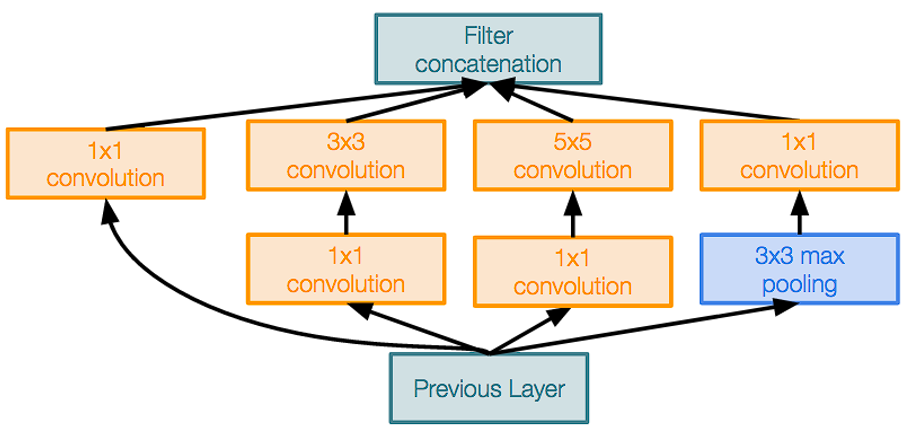
\includegraphics[scale=0.3]{Inception.png}
  \caption{Inception模块基本结构}
  \label{fig-Inception}
\end{figure}

在一般的神经网络中,一层只能表示卷积层或者池化层,而且卷积层的卷积核具有固定的大小. 但是,实际情况下,对于不同尺度的图片,使用不同大小的的卷积核,识别的效果可能各不相同,因为感受野都不同,所以我们希望让神经网络自动去选择效果好的卷积核大小,于是一个Inception模块中\textbf{并列了多种不同的卷积核操作},神经网络可以通过调节参数自适应选择卷积核大小.

但是直接并列卷积核会导致参数数目大大增加,特征图厚度(即通道数个数)太大,为解决该问题,加入$1\times 1$的卷积核减少特征图厚度(也称瓶颈层,Bottleneck). 这样就可以大大减少参数数量,并且增加的$1\times 1$卷积在降维之后可以更加有效、直观地进行数据的训练和特征提取.

为了避免梯度消失,GoogleNet使用了两个辅助分类器接受中间结点的loss值,但是后面发明的batch归一化操作可以代替这个部分.

GoogleNet总层数为22层,而VGG总层数为19层,但是GoogleNet的模型使用内存仅为VGG的$1/10$.

\subsubsection{ResNet}

残差神经网络(ResNet)是2015年ImageNet比赛的第一名,其层数直接增加到了152层. 参考论文\href{https://arxiv.org/pdf/1512.03385.pdf}{Deep Residual Learning for Image Recognition - 2015}.

ResNet主要成就在于发现了“退化现象(Degradation)”,针对退化现象发明了“快捷连接(Shortcut connection)”极大程度的缓解了深度过大的神经网络训练问题.

如果一个神经网络在浅层就能完成图像分类问题,那么一定可以利用更深层的神经网络完成相同的任务,主需要将浅层神经网络后面加入多层恒等变换层即可.

但实验发现事实并不如此,使用深层神经网络在准确率达到某一个饱和值后迅速下降,该过程被ResNet团队称为“退化现象”,他们将发生这种退化现象的原因归结为深层神经网络难以实现“恒等变换”操作. 这里是因为,神经网络使用大量非线性转换将数据映射到高维空间一遍完成更好的分类,导致数据变得更加离散,此时数据已经难以回到原始状态(恒等变换),所以发生“退化现象”.

解决“退化现象”的方法就是将线性变换与非线性变换进行平衡,于是ResNet中引入ResNet模块增加了“快捷连接”分支,期望让网络自动地在线性变换和非线性变换之间寻找平衡. ResNet模块如图\ref{fig-ResNet}所示.
\begin{figure}[htbp]
  \centering
  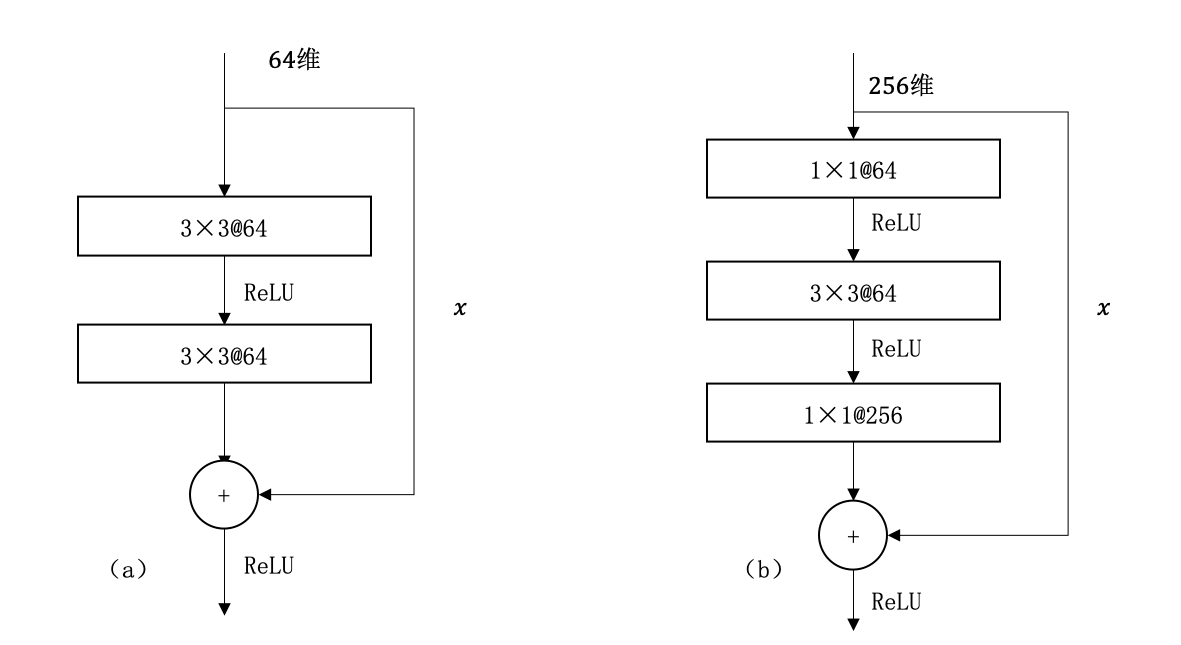
\includegraphics[scale=0.8]{ResNet模块.png}
  \caption{ResNet模块}
  \label{fig-ResNet}
\end{figure}

ResNet模块分为两种:ResNet构建块(a),降采样的ResNet构建块(b). 降采样的构建块即在主干分支上增加了一个$1\times 1$的卷积核(瓶颈层),和GoogleNet在Inception模块中使用的相同,减少参数个数同时增加卷积层,增强提取特征的能力.

\subsubsection{MobileNet}
MobileNet是Google于2017年提出的神经网络,经典轻量级神经网络,参考论文:\href{https://arxiv.org/pdf/1704.04861.pdf}{MobileNets: Efficient Convolutional Neural Networks for Mobile Vision Applications - 2017}.

轻量级神经网络是专注于在移动设备上运行的神经网络,主要思路有两个方向:1. 对训练好的复杂模型进行压缩得到较小的模型;2. 直接设计较小而模型进行训练. 其目的是保持模型性能(Accuracy)的前提下降低模型大小(Parameters Size),同时提升模型速度(Speed, Low Latency). MobileNet牺牲了少量的精度和但是极大地提升了的速度和降低了模型大小.

MobileNet的核心思想就是将标准卷积转化为\textbf{深度可分离卷积},具体原理参考了\href{https://zhuanlan.zhihu.com/p/70703846}{知乎-轻量级神经网络MobileNet}中的解释:将原有卷积操作分为两个部分,\textbf{深度卷积和逐点卷积},如图\ref{fig-MobileNet}所示
\begin{figure}[htbp]
  \centering
  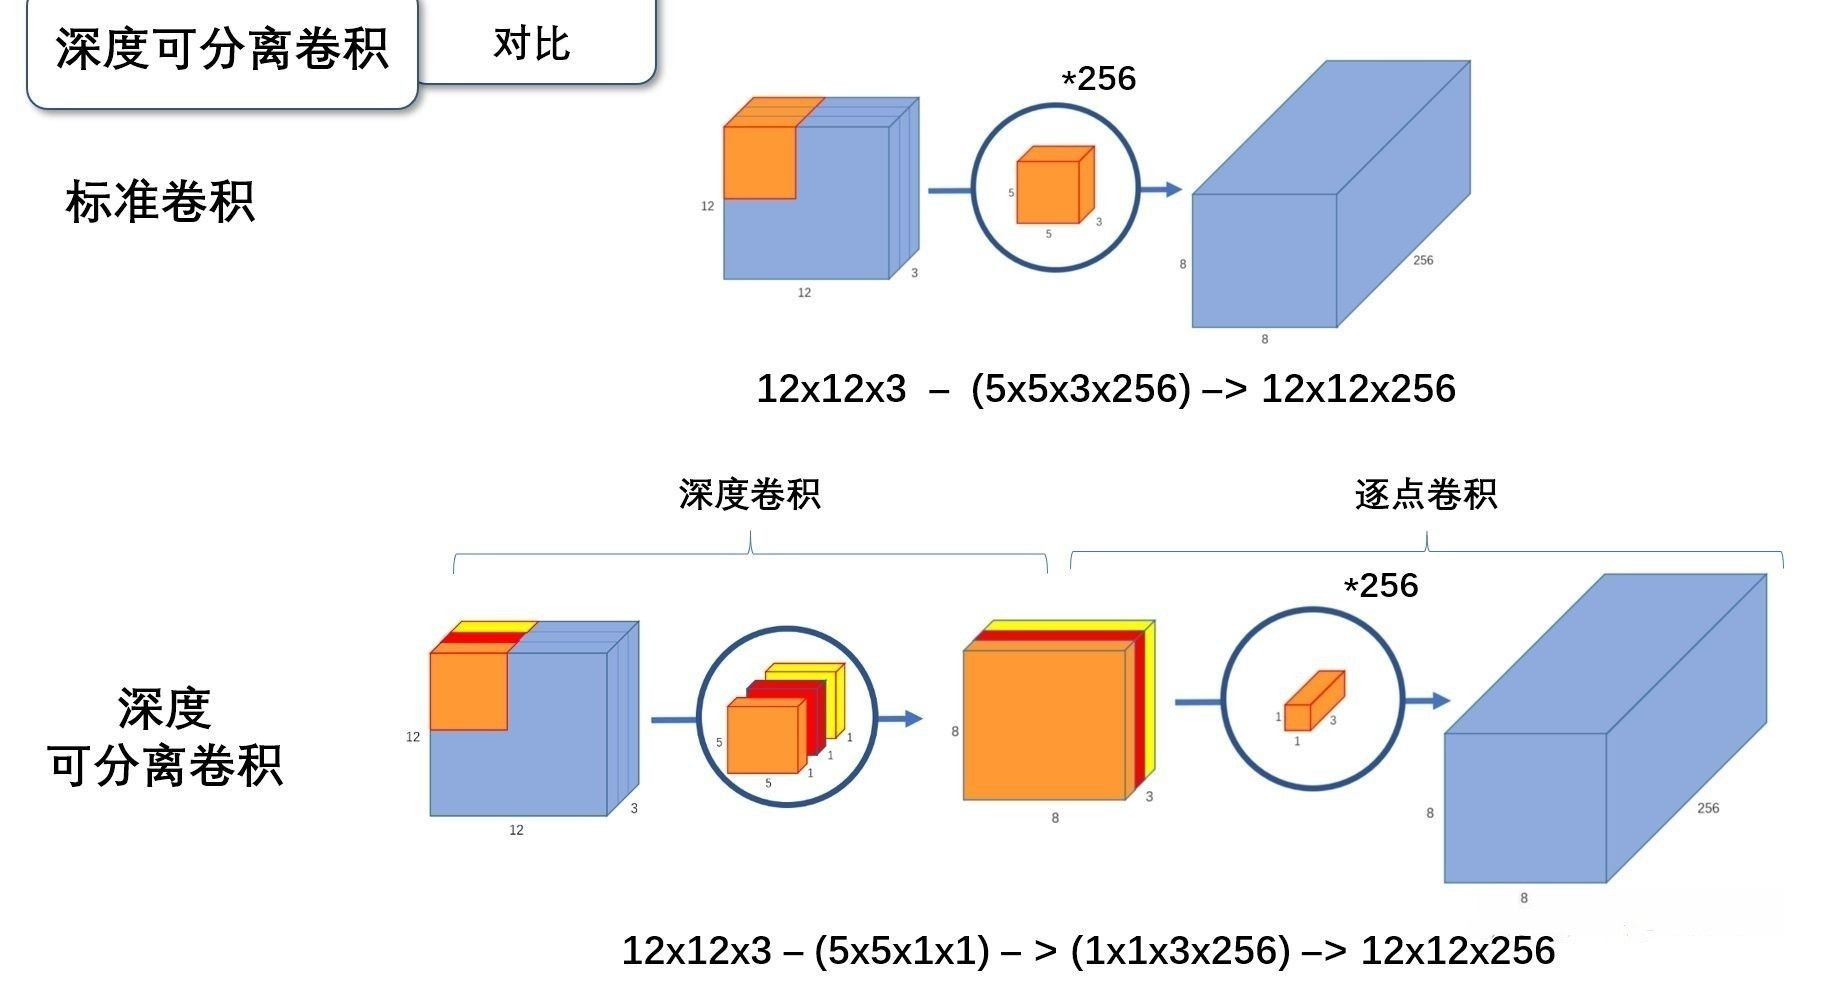
\includegraphics[scale=0.4]{深度可分离卷积.jpg}
  \caption{标准卷积和深度可分离卷积对比}
  \label{fig-MobileNet}
\end{figure}

深度可分离卷积与标准卷积不同的是:我们将卷积拆分为多层单通道形式,不改变图像深度的情况下,先对每一通道进行卷积操作,这样特征图像保持和输入图像相同的通道数目;然后使用逐点卷积,也就是$1\times 1$卷积(就是之前在GoogleNet、Resnet中都是用过的瓶颈层,只不过这次是可以用于升维),我们使用多通道的$1\times 1$的卷积核作用在刚才输出的特征图像上,即可得到和标准卷积相同大小的特征图像结果.

与之不同的是,深度可分离卷积具有更小的量和计算量,设原始图像通道数为$M$,卷积核大小为$D_k\times D_k\times M\times N$,输出的特征图像大小为$D_W\times D_H\times N$. 则标准卷积的参数数目和计算次数分别为:$D_K\times D_K\times M\times N$,$D_K\times D_K\times M\times N\times D_W\times D_H$,而可分离卷积的参数数目和计算次数分别为:\add $(D_K\times D_K+N)\times M$,$(D_K\times D_K+N)\times M\times D_W\times D_H$,\add 于是我们发现深度可分离卷积在参数数目和计算速度上都减少了$\frac{1}{N}+\frac{1}{D_K\times D_K}$($N$一般较大,所以主要由第二项控制大小). 如果我们将卷积取为$3\times 3$,则整体速度提升大约$9$倍!

经过实验发现,MobileNet在ImageNet数据库上的准确率仅比VGG16低$0.9\%$,而参数量减少了$30$倍.

\subsubsection{EfficientNet}
EfficientNet是Google于2019年提出的神经网络,参考论文:\href{https://arxiv.org/pdf/1905.11946v5.pdf}{EfficientNet: Rethinking Model Scaling for Convolutional Neural Networks - 2019}.

在之前ImageNet比赛中我们可以看出,通过对网络的不断扩展可以提高网络的性能,具体扩展方向有如下三个(如图\ref{fig-EfficientNet}所示):
\begin{enumerate}
  \item 增加网络层数
  \item 增加网络宽度
  \item 高分辨率
\end{enumerate}
\begin{figure}[htbp]
  \vspace*{-0.5cm}
  \hspace*{-2cm}
  \centering
  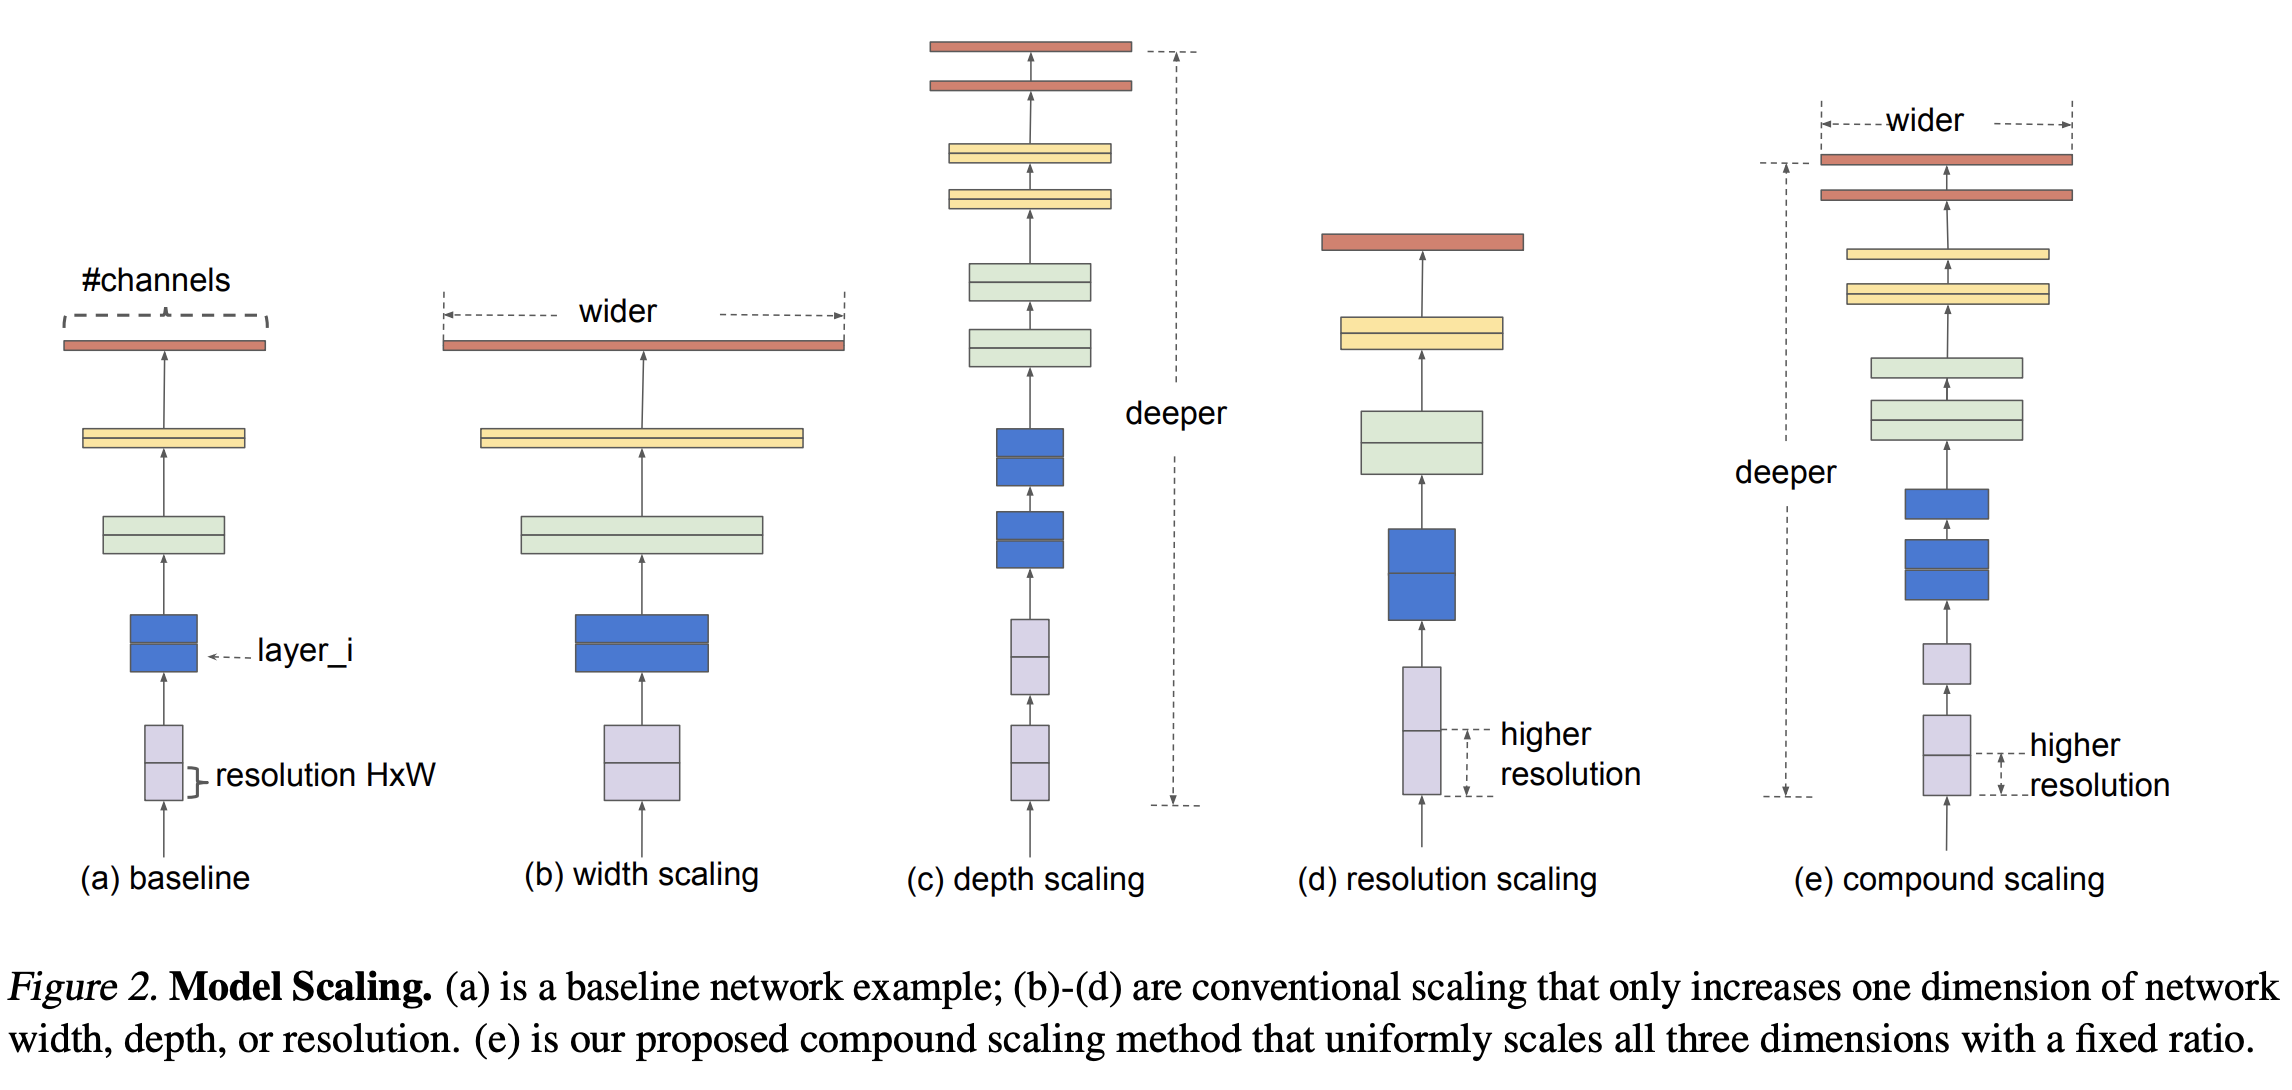
\includegraphics[scale=0.5]{EfficientNet.png}
  \caption{EfficientNet基本结构}
  \label{fig-EfficientNet}
\end{figure}

具体思路是通过神经网络求解平衡三个参数之间的关系,使精度和效率最大化,具体实现较为复杂不再详细分析. 实验表明EfficientNet在迁移学习上也具有很好的表现,在实际效果上优于之前的经典网络,如下图\ref{fig-compare}所示
\begin{figure}[htbp]
  \hspace*{-2cm}
  \centering
  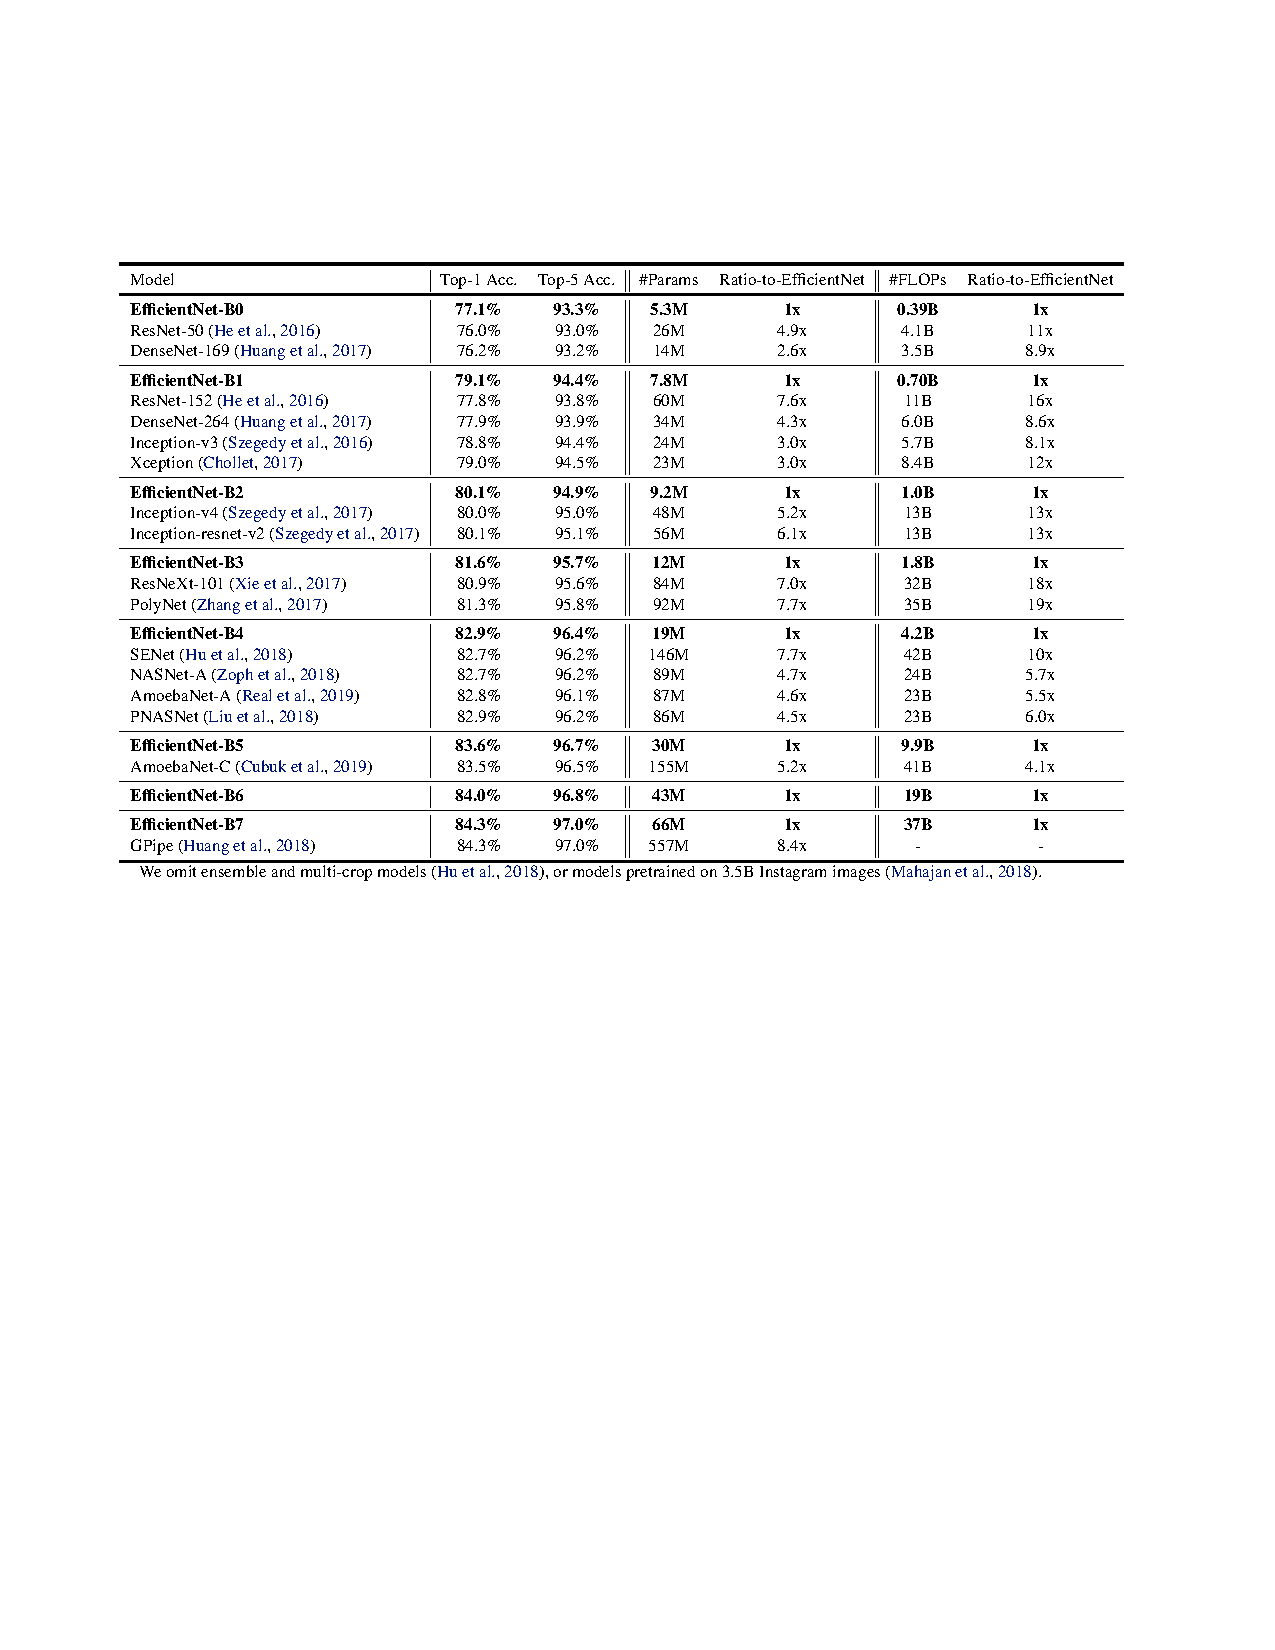
\includegraphics[scale=1.15]{EfficientNet.pdf}
  \caption{EfficientNet与其他网络比较}
  \label{fig-compare}
\end{figure}

\section{实验步骤与结果分析}
我们使用Pytoch对VGG-19模型进行搭建,并进行了训练,模型搭建
\section{结论与讨论}
\end{document}